\documentclass[10pt,twocolumn]{article}
\usepackage{times}
\usepackage{multirow}
\usepackage{graphicx,grffile}
\usepackage{pgf}
\usepackage{tikz}
\usetikzlibrary{arrows,automata}
\usepackage[latin1]{inputenc}

% do not change these values
\baselineskip 12pt
\textheight 9in
\textwidth 6.5in
\oddsidemargin 0in
\topmargin 0in
\headheight 0in
\headsep 0in

%\makeatletter
%\def\maxwidth{\ifdim\Gin@nat@width>\linewidth\linewidth\else\Gin@nat@width\fi}
%\def\maxheight{\ifdim\Gin@nat@height>\textheight\textheight\else\Gin@nat@height\fi}
%\makeatother
%% Scale images if necessary, so that they will not overflow the page
%% margins by default, and it is still possible to overwrite the defaults
%% using explicit options in \includegraphics[width, height, ...]{}
%\setkeys{Gin}{width=\maxwidth,height=\maxheight,keepaspectratio}
%

\usepackage[unicode=true]{hyperref}
\hypersetup{breaklinks=true,
            bookmarks=true,
            pdfauthor={},
            pdftitle={},
            colorlinks=true,
            citecolor=blue
            urlcolor=blue,
            linkcolor=blue,
            pdfborder={0 0 0}}
\urlstyle{same}  % don't use monospace font for urls

\usepackage[font=footnotesize,labelfont=bf]{caption}

\begin{document}

\title{title}

\author{
%Noah Watkins, Neha Ojha\textsuperscript{*}, Carlos Maltzahn \\
%\small {\em University of California, Santa Cruz} \\
%\small {\{jayhawk,carlosm\}@cs.ucsc.edu} \textsuperscript{*}nojha@ucsc.edu \\ [2mm]
\small Submission Type: Research
}

\date{}
\maketitle

\begin{abstract}
abstract
\end{abstract}

\section{Introduction}

\begin{figure}[h]
  \centering
    \includegraphics[width=0.45\textwidth]{experiments/objclass-dev/output.png}
    \caption{
[\href{https://github.com/noahdesu/zlog-popper/tree/master/experiments/objclass-dev/visualize.ipynb}{source}]
Growth of officially supported, custom object interfaces in RADOS over 6
years. A \emph{method} is a specific object interface and a \emph{class} is a
logical grouping of methods.
}
\end{figure}

\section{Storage System Programmability}

When application goals are not met by a storage system the most common reaction
is to design a workaround. Workarounds roughly fall into one of two categories:
so called ``bolt-on'' services that introduce a 3rd party system (e.g. a
metadata service), or expanded application responsibility in the form of data
management (e.g. a new data layout).

\begin{table}
\begin{tabular}{|l|l|l|}
\hline
Category & Specialization & Methods \\ \hline
\multirow{2}{*}{Locking} & Shared & \multirow{2}{*}{6} \\
                         & Exclusive & \\ \hline
\multirow{3}{*}{Logging} & Replica & 3 \\
                         & State & 4 \\
                         & Timestamped & 4 \\ \hline
Garbage Collection & Reference Counting & 4 \\ \hline
\multirow{4}{*}{Metadata Management} & RBD & 37 \\
 & RGW & 27 \\
 & User & 5 \\
 & Version & 5 \\ \hline
\end{tabular}
\caption{A variety of RADOS object storage classes exist that expose reusable interfaces to applications.}
\label{tab:objclasses}
\end{table}

\section{Consolidated Section}

Up until this point we have introduced Ceph, CORFU, the general problems
associated with programmability, described ZLog as being an instantiation of
the CORFU interface on top of Ceph.

Template for the CORFU object class interface. Maybe a simple state machine.

Describe indexing and protocol enforcement.
Differences between built-in interfaces and custom cls interfaces.

\begin{figure}
\centering
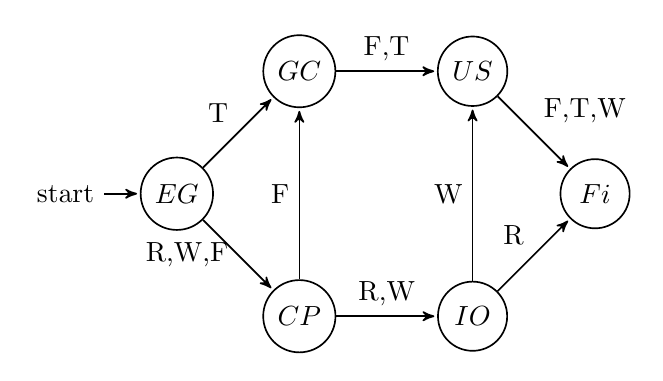
\begin{tikzpicture}[->,>=stealth',shorten >=1pt,auto,node distance=2.2cm,semithick]
%\tikzstyle{every state}=[fill=red,draw=none,text=white]

  \node[initial left,state] (A)              {$EG$};
  \node[state]         (B) [below right of=A] {$CP$};
  \node[state]         (D) [right of=B]       {$IO$};
  \node[state]         (C) [above right of=A] {$GC$};
  \node[state]         (E) [right of=C]       {$US$};
  \node[state]         (F) [below right of=E] {$Fi$};

  \path (A) edge        node [left] {R,W,F} (B)
            edge        node {T}     (C)
        (B) edge        node {F}     (C)
            edge        node {R,W}   (D)
        (C) edge        node {F,T}   (E)
        (D) edge        node {W}     (E)
            edge        node {R}     (F)
        (E) edge        node {F,T,W} (F);
\end{tikzpicture}
\caption{State transition diagram for read ($R$), write ($W$), fill ($F$), and
trim ($T$) CORFU operaitons. The states epoch guard ($EG$), check position ($CP$),
and update state ($US$) access metadata. The I/O performs a log entry read or
write, and garbage collection ($GC$) marks entries for reclamation.}
\end{figure}

\section{ZLog Physical Design}

In this section we examine the design space for mapping the CORFU protocol onto
the RADOS storage system. Recall from Section X the options for rados,
and from section Y for corfu options. The cross product forms the design space.
Want to winnow this down.

\subsection{Storage Interface Selection}

\begin{table}
\begin{tabular}{ | l | l | l | l | l |}
\hline
Map & I/O & Entry Size & Addressing & Metadata \\ \hline
\multirow{2}{*}{1:1} & KV  & Flex     & Ceph      & KV/BS \\ \cline{2-5}
                     & BS  & Flex     & Ceph/VFS  & KV/BS \\ \hline
\multirow{4}{*}{N:1} & KV  & Flex     & \multicolumn{2}{|c|}{KV/BS} \\ \cline{2-5}
                     & WR  & Fixed    & VFS       & KV/BS \\ \cline{2-5}
                     & AP  & Flex     & KV/BS     & KV/BS \\
\hline
\end{tabular}
\caption{The high-level design space of mapping CORFU log entry storage onto
the RADOS object storage system.}
\label{t:init-ds}
\end{table}

Constructing a complete implementation for each configuration would take
a lot of time, and may be time wasted if some configurations can be shown
to never be a viable option.

To winnow down the design space we ran a set of benchmarks---one for each
configuration--- that stressed the raw write performance using the built-in,
optimized interfaces on an unmodified version of Ceph. We explicitly avoided
simulating the costs associated with indexing or protocol enforcement in order
to form a clean baseline. Log entries may vary in size depending on the
application, but per-entry metadata is constant.

\begin{figure}[h]
  \centering
  \includegraphics[width=0.45\textwidth]{experiments/librados-sweep/output.soft.reset.png}
  \caption{
[\href{https://github.com/noahdesu/zlog-popper/tree/master/experiments/librados-sweep/visualize.ipynb}{source}]
Throughput (IOPS) of 1K writes to a single OSD using the standard I/O
interfaces in various configurations. The best performance is achieved using
the byte stream interface and a N:1 mapping strategy.
}
\end{figure}


The first thing to notice is that the configurations using a 1:1 mapping
perform poorly relative to the other configurations. This is unfortunate
because a 1:1 mapping simplifies data management by avoiding the need to
multiplex entries onto a smaller set of objects. However, even if performance
was acceptable, notice that throughput dramatically drops in the tail when the
number of objects reaches a threshold forcing the object cache to spill to
disk. Note that in a large cluster this mode may take a long time reach,
but we avoid it due to the inherent risk.

The KV/N:1 is a convenient configuration because the key-value interface
can be used to easily address log entries and manage index data. However, the
performance of KV/N:1 can vary widely depending on the size of the data entry.
As we will see next, even though the KV/N:1 configuration simplifies data
management, small entry performance falls behind that of N:1 configurations
that store data in the stream interface.

\begin{figure}[h]
  \centering
  \includegraphics[width=0.45\textwidth]{experiments/basic-cls-rand-read/output.read.60min.png}
  \caption{
[\href{https://github.com/noahdesu/zlog-popper/tree/master/experiments/basic-cls-rand-read/visualize.ipynb}{source}]
Throughput of 1K random reads to a single OSD using the standard I/O
interfaces in various configurations. The best performance is achieved using
the byte stream interface and a N:1 mapping strategy.
}
\end{figure}


Figure \ref{f:librados-sweep} shows the single-node write-only I/O throughput
for each of the points in the design space defined in Table \ref{t:init-ds}.
The results reveal poor relative performance using both the key-value storage
interface, as well as either of the 1:1 strategies---which incur overhead by
creating a new object for each log entry. Both of the N:1 strategies using the
bytestream I/O interface outperform all of the other approaches by over 2x
throughput, but otherwise have nearly identical performance. As a first
approximation these results show that when optimizing for log append throughput
the design space should be refined by limiting solutions to architectures based
on a N:1 mapping strategy using the bytestream I/O interface.

To examine the read performance of the points in the design space we generated
a dataset using each of the write workloads, and then issued random reads
across the entire dataset. Figure \ref{f:librados-rand-read} shows the read
throughput for each of the design strategies. The results show that an N:1
mapping using bytestream interface performs best. Interestingly, the 1:1
mapping strategy using the bytestream interface exhibits good read performance
in comparison to writes using the same strategy.

The configurations based on bytestream storage exhibit the best performance.
The *write* variation depends on client-side mapping to object offset and
indirectly on the VFS index layer within the OSD, but this method is
incompatible with non-fixed size entries. Alternatively, the *append* variation
supports both fixed and dynamic size entries, but leaves the indexing and
protocl enforcment challenges unsolved.

In conclusion, both *write* and *append* variation of bytestream configurations
are the best choice, with an edge given to *append* if it can support dynamic
sized entries without sacrificing performance.

\subsection{Metadata Management}

\begin{figure}[h]
  \centering
  \includegraphics[width=0.45\textwidth]{experiments/basic-cls-overhead/output.1024.soft.reset.png}
  \caption{
[\href{https://github.com/noahdesu/zlog-popper/tree/master/experiments/basic-cls-overhead/visualize.ipynb}{source}]
}
\end{figure}

Many variations of design here. What is the easiest way to 
winnow down the design space.

NEXT GRAPH A

This is an easy interface to simulate.
- Check Epoch (omap, stream header)
- this graph also has the APPEND raw through for comparison
- adds NEW OSD OP TO AVOID CLS OVERHEAD DISCUSSION FOR PAPER
- 3 runs in this graph, no need to write interface
- short runs to verify and then do all long runs togther with next graph

Both protocol enforcement and logical address translation
represent a larger design space involving index design. However
since in either case all state must be stored in the omap and
in the stream header, testing the overhead of epoch enforcement
provides a strict upper bound on performance.

- Protocol Enforcement
- Logical Translation (only append case)

Memory Cache

NEXT GRAPH B (or combined with A)
Use in-memory cache to implement the epoch check and show that we can match
the raw performance even with this added functionality.
This will show the content from graph A for comparison. Look
we match the raw performance.

NEXT GRAPH B or C (probably just two).. bar chart?
 Final consolidation of average throughputs of all the different
methods
 THIS INCLUDES THE FULL IMPL OF ZLOG APPEND using the in-memory cache

We solve the slow down of the epoch by storing the value in memory. Here is
the new performance.  We are able to with the epoch check match the raw
performance.

We know that we cannot use kv/bs for logicla address translation or protocol
enforcement without a performance hit so there is no point in trying. instead,
we generalize this memory cache hting used for epoch checks as a
new interface and use this interface to implement the full zlog
stack and show the performance.

Overall corfu is relatively simple abtraction, yet requires significant
work in making performant. Further, the decision may change over time.

We will probably have room in the paper to discuss the design of the
index structure, like collapsing a bit map and taking advantage of
the implicit strides in the offsets, etc... but we can probably move
that to a later section to keep this presentation concise. We should
probably mention this aspect here, but overall that becomes a ortholognal
optimization.

%# Abstract Model

%# Sequencer Creation

\end{document}
